\documentclass[12pt,a4paper]{article}
\usepackage[utf8]{inputenc}
\usepackage[T1]{fontenc}
\usepackage{geometry}
\usepackage{setspace}
\usepackage{graphicx}
\usepackage{booktabs}
\usepackage{longtable}
\usepackage{array}
\usepackage{hyperref}
\usepackage{enumitem}
\usepackage{float}
\usepackage{tikz}
\usetikzlibrary{arrows.meta, positioning, shapes.geometric}
\geometry{margin=1in}
\setstretch{1.25}

\title{Fake News Detection using Machine Learning and Deep Learning}
\author{Ayman El Ouardiji \and Ilyas El Alaoui Saleh}
\date{\today}

\begin{document}

\maketitle
\thispagestyle{empty}
\newpage

\begin{abstract}
This project presents a complete fake news detection system built with both classical machine learning and deep learning techniques. The work uses the Kaggle dataset \texttt{clmentbisaillon/fake-and-real-news-dataset}, prepares a unified labeled dataset, applies NLP preprocessing, trains three TF-IDF based classifiers and one LSTM model, compares all models with the same evaluation protocol, selects the best model automatically, and deploys it through a FastAPI backend and a Streamlit interface. The final verified results show that the Linear Support Vector Machine achieved the best F1-score of 0.9984 on the held-out test set, outperforming Logistic Regression, Multinomial Naive Bayes, and the LSTM baseline on this dataset. The system therefore demonstrates both academic value and practical deployment readiness.
\end{abstract}

\newpage

\section{Introduction}
Fake news detection has become an important problem in natural language processing because misleading content can spread rapidly and influence political opinion, social trust, and public understanding. Since misinformation is often written in a style that resembles legitimate reporting, it cannot be detected reliably with simple keyword rules. It requires a supervised classification pipeline that can learn statistical patterns from real and fake news articles.

In this project, fake news detection is treated as a binary text classification task with two labels: \texttt{FAKE} and \texttt{REAL}. The work compares classical machine learning approaches with a deep learning approach under the same data preparation and evaluation process. In addition, the project is not limited to model training only. It also includes dataset preparation, saved artifacts, automatic best-model selection, an API service, and a web interface, making it a complete end-to-end system.

\section{Project Objectives}
The main objectives of the project are:
\begin{itemize}[leftmargin=*]
\item prepare a usable training dataset from the Kaggle source files,
\item preprocess English news text in a consistent way,
\item train and compare multiple machine learning and deep learning models,
\item evaluate all models with suitable classification metrics,
\item select the best model automatically using F1-score,
\item deploy the selected model through FastAPI and Streamlit,
\item document the whole process clearly for academic presentation.
\end{itemize}

\section{Authors}
This project was carried out by:
\begin{itemize}[leftmargin=*]
\item Ayman El Ouardiji
\item Ilyas El Alaoui Saleh
\end{itemize}

\section{Dataset Description}
\subsection{Dataset Source}
The system uses the Kaggle dataset \texttt{clmentbisaillon/fake-and-real-news-dataset}. This dataset contains two original CSV files:
\begin{itemize}[leftmargin=*]
\item \texttt{True.csv} containing real news articles,
\item \texttt{Fake.csv} containing fake news articles.
\end{itemize}

\subsection{Dataset Preparation}
A dedicated script named \texttt{src/prepare\_dataset.py} downloads the dataset using \texttt{kagglehub}, loads both CSV files, creates a new label column, and concatenates them into one local file named \texttt{data/fake\_news\_dataset.csv}.

The label assignment is:
\begin{itemize}[leftmargin=*]
\item rows from \texttt{True.csv} receive the label \texttt{REAL},
\item rows from \texttt{Fake.csv} receive the label \texttt{FAKE}.
\end{itemize}

\subsection{Dataset Schema}
The merged dataset contains the following columns:
\begin{itemize}[leftmargin=*]
\item \texttt{title}
\item \texttt{text}
\item \texttt{subject}
\item \texttt{date}
\item \texttt{label}
\end{itemize}

\subsection{Verified Size}
The merged raw dataset contains 44,898 rows. During the training pipeline, missing and empty rows are removed. After cleaning, 44,267 rows are used for model training and evaluation.

\begin{table}[H]
\centering
\caption{Dataset summary after preparation and cleaning}
\begin{tabular}{lc}
\toprule
Description & Value \\
\midrule
Raw merged rows & 44,898 \\
Rows after cleaning & 44,267 \\
FAKE rows after cleaning & 22,851 \\
REAL rows after cleaning & 21,416 \\
Training text column & \texttt{text} \\
Training label column & \texttt{label} \\
\bottomrule
\end{tabular}
\end{table}

\section{System Workflow}
The overall workflow of the project is shown in Figure~\ref{fig:global-workflow}. It starts from dataset download and ends with a deployed prediction system.

\begin{figure}[H]
\centering
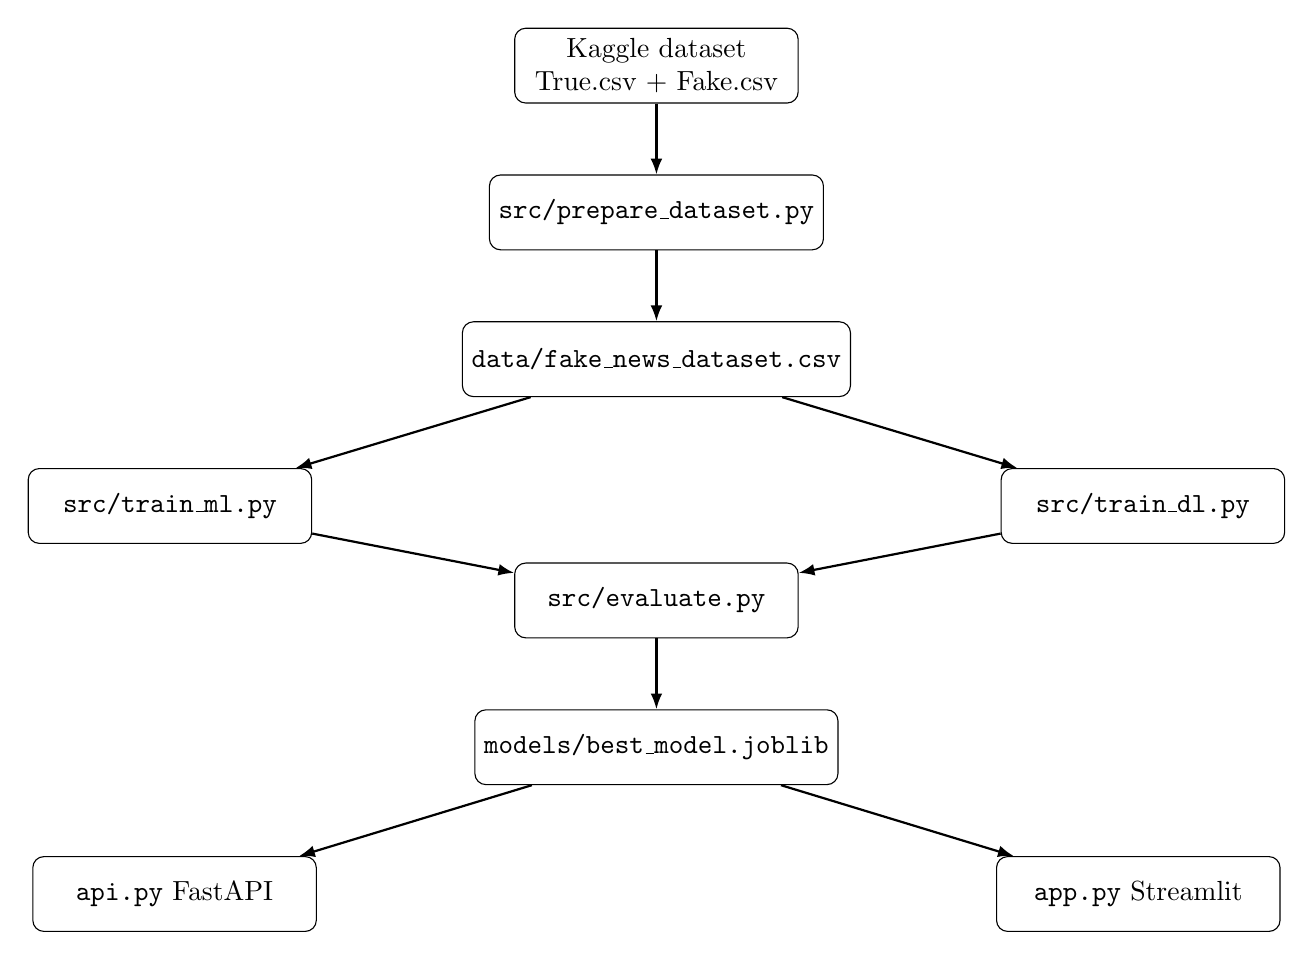
\begin{tikzpicture}[
node distance=0.9cm and 0.7cm,
box/.style={rectangle, rounded corners, draw=black, align=center, minimum width=3.6cm, minimum height=0.95cm},
line/.style={-{Latex[length=2mm]}, thick}
]
\node[box] (kaggle) {Kaggle dataset\\True.csv + Fake.csv};
\node[box, below=of kaggle] (prepare) {\texttt{src/prepare\_dataset.py}};
\node[box, below=of prepare] (csv) {\texttt{data/fake\_news\_dataset.csv}};
\node[box, below left=of csv, xshift=-1.2cm] (ml) {\texttt{src/train\_ml.py}};
\node[box, below right=of csv, xshift=1.2cm] (dl) {\texttt{src/train\_dl.py}};
\node[box, below=2.1cm of csv] (eval) {\texttt{src/evaluate.py}};
\node[box, below=of eval] (best) {\texttt{models/best\_model.joblib}};
\node[box, below left=of best, xshift=-1.3cm] (api) {\texttt{api.py} FastAPI};
\node[box, below right=of best, xshift=1.3cm] (app) {\texttt{app.py} Streamlit};

\draw[line] (kaggle) -- (prepare);
\draw[line] (prepare) -- (csv);
\draw[line] (csv) -- (ml);
\draw[line] (csv) -- (dl);
\draw[line] (ml) -- (eval);
\draw[line] (dl) -- (eval);
\draw[line] (eval) -- (best);
\draw[line] (best) -- (api);
\draw[line] (best) -- (app);
\end{tikzpicture}
\caption{Global workflow of the fake news detection system}
\label{fig:global-workflow}
\end{figure}

\section{Preprocessing}
\subsection{Cleaning Steps}
The preprocessing stage normalizes text before feature extraction. The following operations are applied:
\begin{enumerate}[leftmargin=*]
\item convert text to lowercase,
\item remove URLs,
\item remove HTML tags,
\item remove punctuation,
\item remove digits,
\item normalize repeated whitespace,
\item tokenize text with NLTK,
\item remove stopwords,
\item apply lemmatization with WordNet.
\end{enumerate}

These steps reduce noise and vocabulary sparsity, which is especially useful for TF-IDF based models and still beneficial before sequence tokenization for the LSTM.

\begin{figure}[H]
\centering
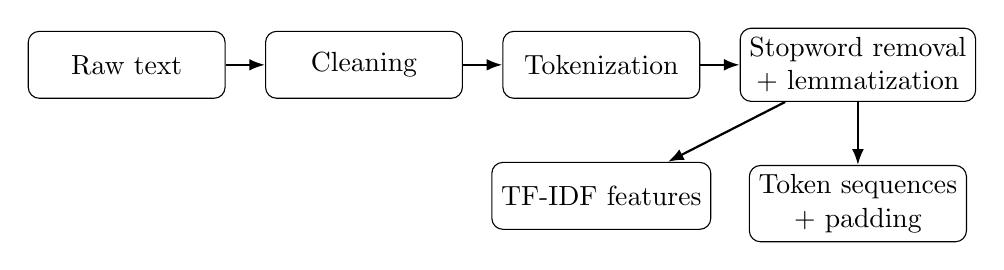
\begin{tikzpicture}[
node distance=0.8cm and 0.5cm,
box/.style={rectangle, rounded corners, draw=black, align=center, minimum width=2.5cm, minimum height=0.85cm},
line/.style={-{Latex[length=2mm]}, thick}
]
\node[box] (raw) {Raw text};
\node[box, right=of raw] (clean) {Cleaning};
\node[box, right=of clean] (tok) {Tokenization};
\node[box, right=of tok] (lemma) {Stopword removal\\+ lemmatization};
\node[box, below=of tok] (tfidf) {TF-IDF features};
\node[box, below=of lemma] (seq) {Token sequences\\+ padding};

\draw[line] (raw) -- (clean);
\draw[line] (clean) -- (tok);
\draw[line] (tok) -- (lemma);
\draw[line] (lemma) -- (tfidf);
\draw[line] (lemma) -- (seq);
\end{tikzpicture}
\caption{Preprocessing pipeline and feature outputs}
\label{fig:preprocessing}
\end{figure}

\section{Machine Learning Models}
Three classical machine learning models are trained:
\begin{itemize}[leftmargin=*]
\item Logistic Regression
\item Linear Support Vector Machine
\item Multinomial Naive Bayes
\end{itemize}

\subsection{Feature Representation}
All classical models use TF-IDF features built from unigrams and bigrams. The vectorizer is configured with:
\begin{itemize}[leftmargin=*]
\item maximum features: 20,000
\item n-gram range: 1 to 2
\item minimum document frequency: 2
\item maximum document frequency: 0.95
\item sublinear term frequency scaling
\end{itemize}

\subsection{Hyperparameter Search}
The classical models are tuned with \texttt{GridSearchCV} using F1-score as the selection metric. The main searched parameters are:
\begin{itemize}[leftmargin=*]
\item \texttt{C} for Logistic Regression
\item \texttt{C} for Linear SVM
\item \texttt{alpha} for Multinomial Naive Bayes
\end{itemize}

\section{Deep Learning Model}
The deep learning part of the project uses an LSTM model implemented with TensorFlow/Keras. The model uses:
\begin{itemize}[leftmargin=*]
\item a tokenizer with a controlled vocabulary,
\item padded integer sequences,
\item an embedding layer,
\item an LSTM layer,
\item dropout,
\item dense layers,
\item a sigmoid output for binary classification.
\end{itemize}

The default training configuration includes:
\begin{itemize}[leftmargin=*]
\item vocabulary size: 20,000
\item maximum sequence length: 300
\item embedding dimension: 128
\item LSTM units: 64
\item batch size: 32
\item epochs: 8
\end{itemize}

\begin{figure}[H]
\centering
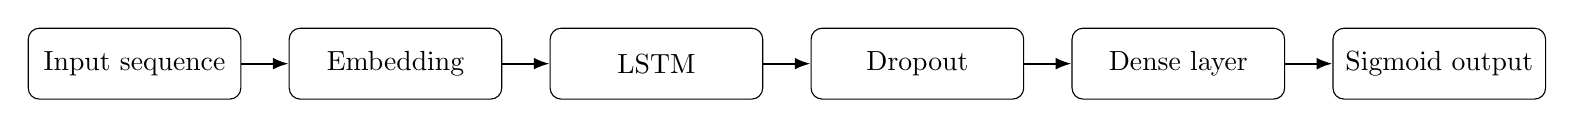
\begin{tikzpicture}[
node distance=0.9cm and 0.6cm,
box/.style={rectangle, rounded corners, draw=black, align=center, minimum width=2.7cm, minimum height=0.9cm},
line/.style={-{Latex[length=2mm]}, thick}
]
\node[box] (input) {Input sequence};
\node[box, right=of input] (embed) {Embedding};
\node[box, right=of embed] (lstm) {LSTM};
\node[box, right=of lstm] (drop) {Dropout};
\node[box, right=of drop] (dense) {Dense layer};
\node[box, right=of dense] (sigmoid) {Sigmoid output};

\draw[line] (input) -- (embed);
\draw[line] (embed) -- (lstm);
\draw[line] (lstm) -- (drop);
\draw[line] (drop) -- (dense);
\draw[line] (dense) -- (sigmoid);
\end{tikzpicture}
\caption{Simplified LSTM architecture used in the project}
\label{fig:lstm-arch}
\end{figure}

\section{Experimental Procedure}
The full experimental procedure was executed in the following order:
\begin{enumerate}[leftmargin=*]
\item install dependencies from \texttt{requirements.txt},
\item prepare the Kaggle dataset with \texttt{src/prepare\_dataset.py},
\item train the classical models with \texttt{src/train\_ml.py},
\item train the LSTM model with \texttt{src/train\_dl.py},
\item aggregate results with \texttt{src/evaluate.py},
\item load the selected model through FastAPI,
\item test the web interface through Streamlit.
\end{enumerate}

The dataset is split with stratified sampling. For the deep learning pipeline, separate training, validation, and test sets are used. For the machine learning pipeline, the combined train and validation portion is used inside grid search, and the final evaluation is reported on the test split.

\section{Evaluation Metrics}
All models are evaluated with the following metrics:
\begin{itemize}[leftmargin=*]
\item Accuracy
\item Precision
\item Recall
\item F1-score
\item Training time
\item Confusion matrix
\end{itemize}

F1-score is used as the main selection metric because fake news detection is a binary classification problem where both false positives and false negatives matter.

\section{Results}
The final measured results are shown in Table~\ref{tab:results}. These values come from the verified execution of the project pipeline.

\begin{table}[H]
\centering
\caption{Final model comparison on the test set}
\label{tab:results}
\begin{tabular}{lccccc}
\toprule
Model & Accuracy & Precision & Recall & F1-score & Training Time (s) \\
\midrule
Linear SVM & 0.998344 & 0.999415 & 0.997375 & 0.998394 & 510.6498 \\
Logistic Regression & 0.996236 & 0.998243 & 0.994457 & 0.996347 & 533.1647 \\
LSTM & 0.993224 & 0.988732 & 0.998250 & 0.993468 & 1555.6750 \\
Naive Bayes & 0.959042 & 0.964664 & 0.955659 & 0.960141 & 417.2454 \\
\bottomrule
\end{tabular}
\end{table}

\subsection{Best Model}
The best model selected automatically by the evaluation script is the Linear SVM. It achieved the highest F1-score of 0.998394 and was therefore exported as the deployment model through \texttt{models/best\_model.joblib}.

\subsection{Interpretation}
The results show that sparse lexical features combined with a linear classifier are extremely effective for this dataset. Even though the LSTM performed strongly, the Linear SVM achieved slightly better overall balance between precision and recall while also being easier to deploy and faster at inference time. This confirms a common observation in text classification: for well-structured supervised datasets, TF-IDF plus a strong linear model can remain highly competitive.

\section{Generated Figures}
The project generates confusion matrices and training curves automatically. The most important figures are included below.

\begin{figure}[H]
\centering
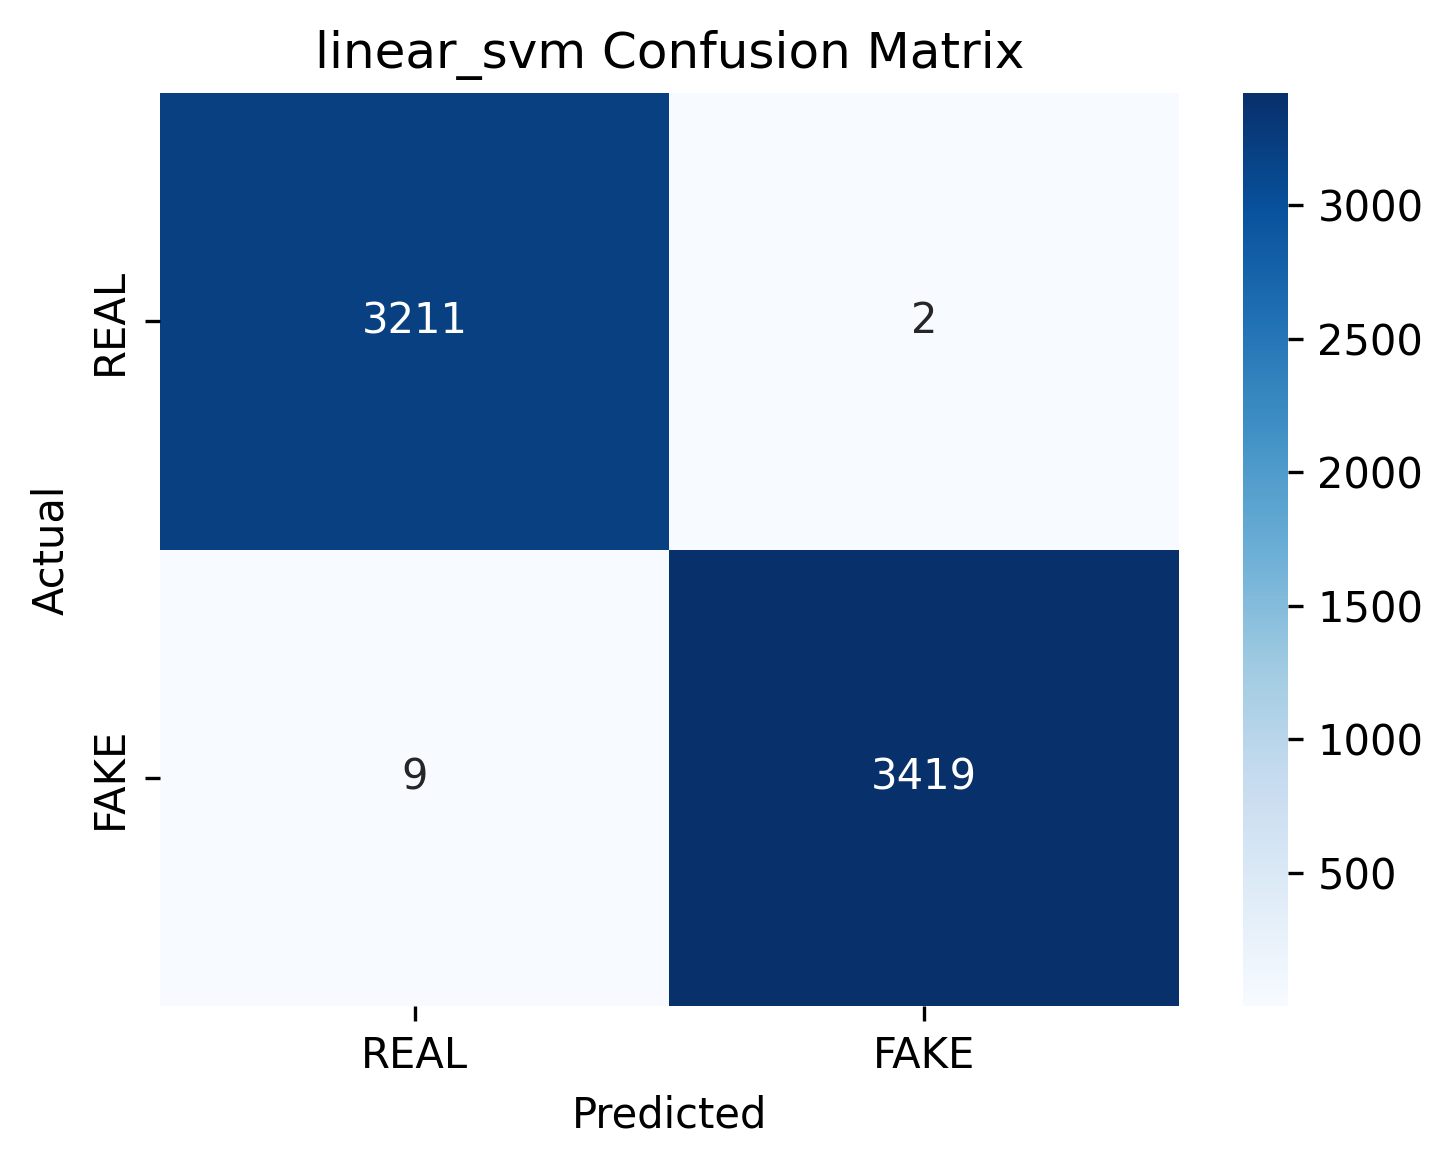
\includegraphics[width=0.72\textwidth]{outputs/figures/linear_svm_confusion_matrix.png}
\caption{Confusion matrix of the best-performing Linear SVM model}
\label{fig:svm-cm}
\end{figure}

\begin{figure}[H]
\centering
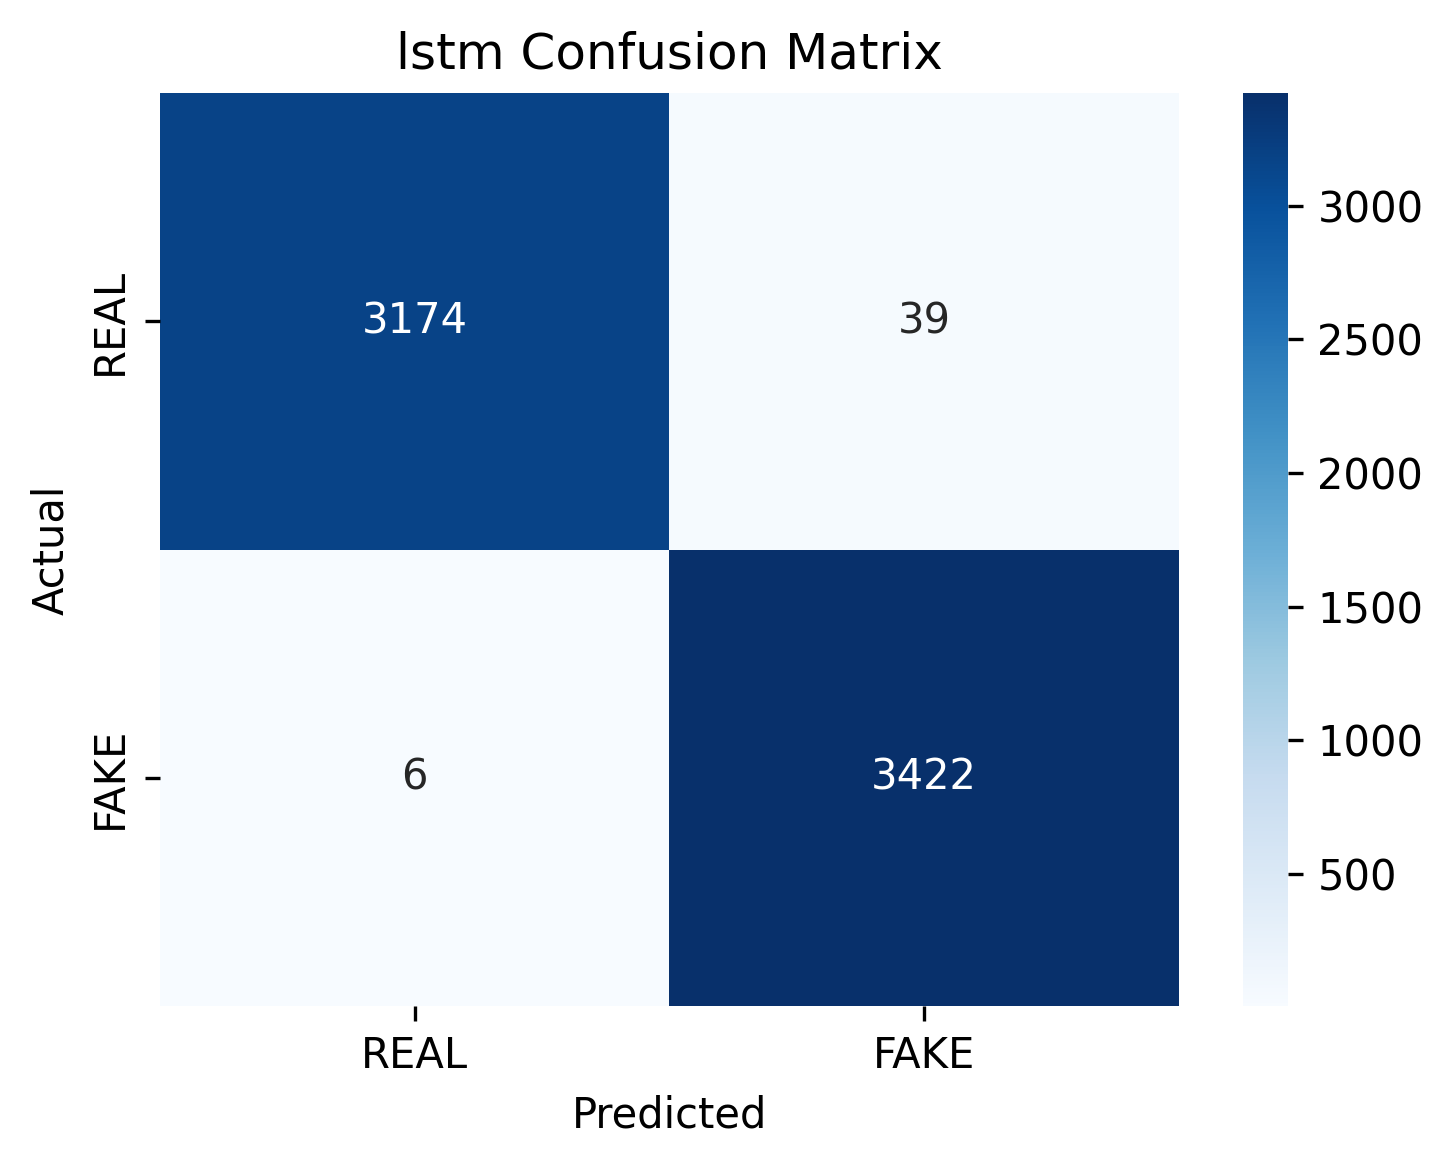
\includegraphics[width=0.72\textwidth]{outputs/figures/lstm_confusion_matrix.png}
\caption{Confusion matrix of the LSTM model}
\label{fig:lstm-cm}
\end{figure}

\begin{figure}[H]
\centering
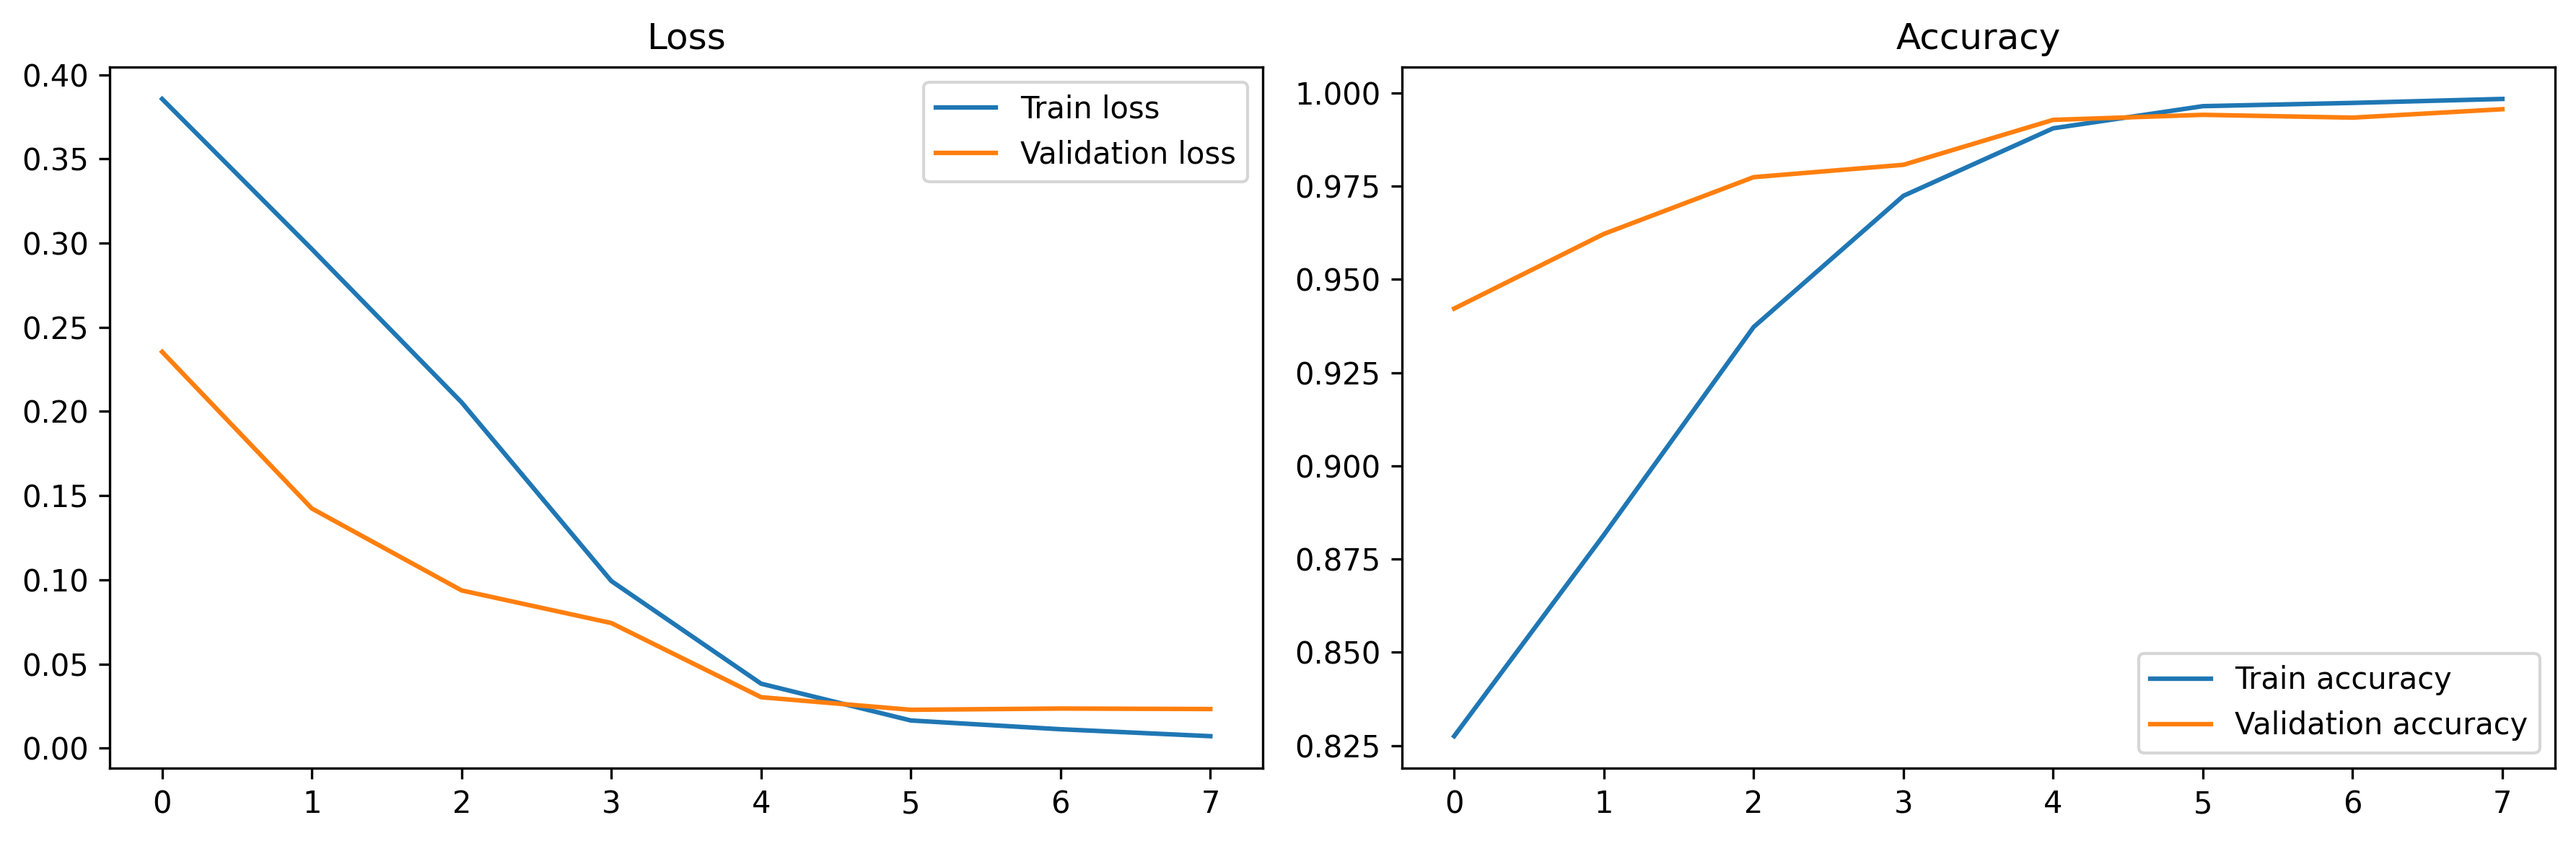
\includegraphics[width=0.88\textwidth]{outputs/figures/lstm_training_curves.png}
\caption{LSTM training curves saved during the verified training run}
\label{fig:lstm-curves}
\end{figure}

\section{Deployment}
\subsection{FastAPI Backend}
The file \texttt{api.py} exposes a prediction endpoint through FastAPI. The backend loads \texttt{models/best\_model.joblib}, reads the referenced model and preprocessing artifacts, preprocesses incoming text, and returns:
\begin{itemize}[leftmargin=*]
\item predicted label,
\item probability of fake news,
\item probability of real news,
\item selected model name.
\end{itemize}

A verified example response produced by the running API is:

\begin{verbatim}
{
  "label": "FAKE",
  "probability_fake": 0.8207,
  "probability_real": 0.1793,
  "model_name": "linear_svm"
}
\end{verbatim}

\subsection{Streamlit Frontend}
The file \texttt{app.py} provides a simple browser interface. A user enters a news paragraph, clicks the analysis button, and receives the classification result from the FastAPI backend. This creates a clean separation between the prediction service and the user interface.

\begin{figure}[H]
\centering
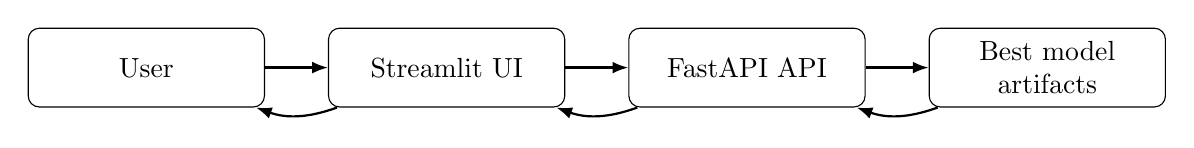
\begin{tikzpicture}[
node distance=1cm and 0.8cm,
box/.style={rectangle, rounded corners, draw=black, align=center, minimum width=3cm, minimum height=1cm},
line/.style={-{Latex[length=2mm]}, thick}
]
\node[box] (user) {User};
\node[box, right=of user] (ui) {Streamlit UI};
\node[box, right=of ui] (api) {FastAPI API};
\node[box, right=of api] (model) {Best model\\artifacts};

\draw[line] (user) -- (ui);
\draw[line] (ui) -- (api);
\draw[line] (api) -- (model);
\draw[line] (model) to[bend left=20] (api);
\draw[line] (api) to[bend left=20] (ui);
\draw[line] (ui) to[bend left=20] (user);
\end{tikzpicture}
\caption{Deployment architecture of the final system}
\label{fig:deployment}
\end{figure}

\section{Practical Issues and Fixes}
During the project validation, several engineering issues were identified and corrected:
\begin{itemize}[leftmargin=*]
\item TensorFlow imports were changed to lazy loading so that the machine learning path and API do not fail when TensorFlow is not needed immediately.
\item The Streamlit configuration line was repaired to remove a malformed page icon string.
\item The default machine learning search settings were adjusted to avoid runaway parallel workers and to complete more reliably on a local machine.
\end{itemize}

These fixes improved reproducibility and made the project easier to run from start to finish.

\section{Conclusion}
This project successfully delivers a complete fake news detection system with both academic and practical value. It begins with a public Kaggle dataset, applies a well-defined preprocessing pipeline, trains multiple classical and neural models, evaluates them with appropriate metrics, selects the best model automatically, and deploys the result through a backend API and a web application.

The strongest result in this project comes from the Linear SVM model with an F1-score of 0.998394. This indicates that, for this dataset, TF-IDF features combined with a linear classifier provide an excellent balance of simplicity, speed, and predictive power. The LSTM model remains a useful deep learning baseline and demonstrates that the system can support neural methods as well.

\end{document}
